\chapter{Services}\label{ch:services}

\section{Traefik Edge Router}\label{sec:traefik}

\begin{figure}[ht]
    \centering
    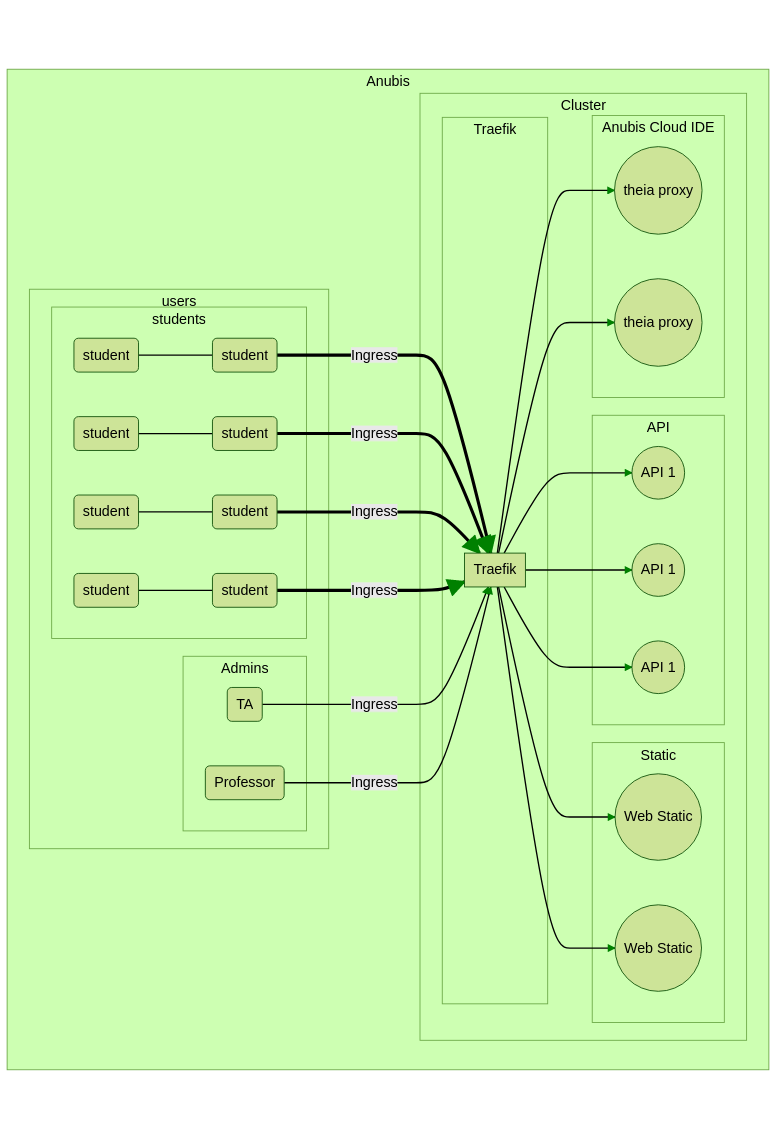
\includegraphics[width=0.5\textwidth]{figures/traefik.mmd}
    \caption{Traefik Traffic in Anubis\label{fig:traefik}}
\end{figure}

For our edge router, we use traefik~\fref{fig:traefik}. 
Traefik will be what actually listens on the servers external ports. 
All external traffic will be routed through Traefik. 
Above all else, we will be using Traefik's powerful routing features to handle the ingress of requests.

Traefik lets us do some spicy and powerful stuff. 
We can route requests to different services based off predefined rules, 
and even change requests as they pass through.

Among other things, the routing rules make it so that we can have 
both the static store and api on the same domain. 
The rules are set up such that every request that 
starts with a path of \textit{anubis.osiris.services/api/*} goes to the api~\fref{sec:api} service.
All other requests \textit{anubis.osiris.services/*} are routed to the web static~\fref{sec:web} service.

In addition to having the web static~\fref{sec:web} and the anubis api~\fref{sec:api} services on
the same domain, we can add routing rules for the theia-proxy~\fref{sec:theia-proxy} service.
Anything that is \textit{ide.anubis.osiris.service/*} will be routed to the theia-proxy service~\fref{sec:theia-proxy}.

By leveraging these features of Traefik, we can make it appear that 
the services work different when being accessed externally.

\section{Anubis API}\label{sec:api}

The API is the backbone of Anubis. 
It is where most of the heavy lifting is done. 
The service relies on both the cache~\fref{sec:caching} and mariadb data 
stores~\fref{sec:data-stores} to maintain state.

The Anubis API is itself nothing more than a simple \href{https://flask.palletsprojects.com/en/2.0.x/}{Flask} app.
As of version \textit{v3.1.16} it is about 25,000 lines of python.

\subsection{Zones}\label{sec:api-zones}

The API is split into two distinct, and uniquely treated zones. 
There is a public and a admin zone.
All endpoints for Anubis fall within one of these zones.
In the source code for Anubis, the views for these zones exist 
in seperate public and admin python modules.

All public view endpoints will start with the url \textit{anubis.osiris.services/api/public/*}.
Similarly, the admin view endpoints will start with \textit{anubis.osiris.services/api/admin/*}.

\subsection{Public Zone}\label{sec:api-public-zone}
The majority of the public API does require authentication.
This is mostly handled by the \textit{@require\_auth} decorator applied to the view function.
Additional checks will be done to verify that the resource, or calculation being requested are
something the requestor (the user making the request) is authorized to see. 
The distinction must be made that public here means that it is public to users.
Students that open Anubis in a web browser and navigate through their submissions and assignments
will only be using the public API.

\subsection{Admin Zone}\label{sec:api-admin-zone}
The admin api zone is where all of the special endpoints that require higher than student level permission reside.
When a TA or Professor uses any functionality of the Admin Panel, they are using these special
admin flask views.
All of the view functions in the admin api module have decorators like \textit{@require\_admin()} or 
\textit{@require\_superuser()}.
These protect the endpoints from anyone without admin permissions on at least one course.
Additional checks are then performed on each endpoint to verify that whatever resource is being requested
or modified is allowed by the current user.

\subsubsection{Course Context}\label{sec:course-context}
Most view functions for the admin api require a \textit{course context} set in the cookie of the request.
When mutli-course management was added to Anubis, most all the view functions for the admin api
needed to be made \textit{"course aware"}. 
What that means is that there needed to be a check that the user making the request is an admin \textit{and} is
an admin for the course that that resource resides under.

\subsection{Health Checks}\label{sec:api-health-checks}
There are very simplistic health checks in the api that make debugging issues much easier.
The endpoint \textit{anubis.osiris.services/} will run the following view funtion:

\begin{minted}{python}
    @app.route("/")
    def index():
        Config.query.all()
        cache_health()
        return "Healthy"
\end{minted}

The view checks that the database~\fref{sec:mariadb} is accessable by running a query, then calls a function that relies on the 
redis cache~\fref{sec:caching}.
While this view function may be simple, it is quite effective.
Most of the incidents of degradded service or downtime come down to either the database or cache being temporary
unavailable.


\subsection{Responsibilites}\label{sec:api-responsibilities}

The Anubis API is responsible for handling most basic 
IO, and state managing that happens on the cluster. 
Some of this includes:

\begin{itemize}
    \item Authenticating users
    \item Providing Class, Assignment, and Submission data to the frontend
    \item Handling github webhooks
    \item Handling reports from the submission pipeline cluster
    \item Handling regrade requests
    \item Initializing new IDE sessions
\end{itemize}

\subsection{Authentication}\label{sec:api-authentication}

To authenticate with the api, a token is required.
The only way to get one of these tokens is through NYU Single Sign On. 
By doing this, we are outsourcing our authentication. 
This saves a whole lot of headaches while being arguably more secure than if we rolled our own.

All of this is about 20 lines on our end. All that is necessary are some keys from NYU IT.

\section{Anubis Web Static}\label{sec:web}

\begin{figure}[ht]
    \centering
    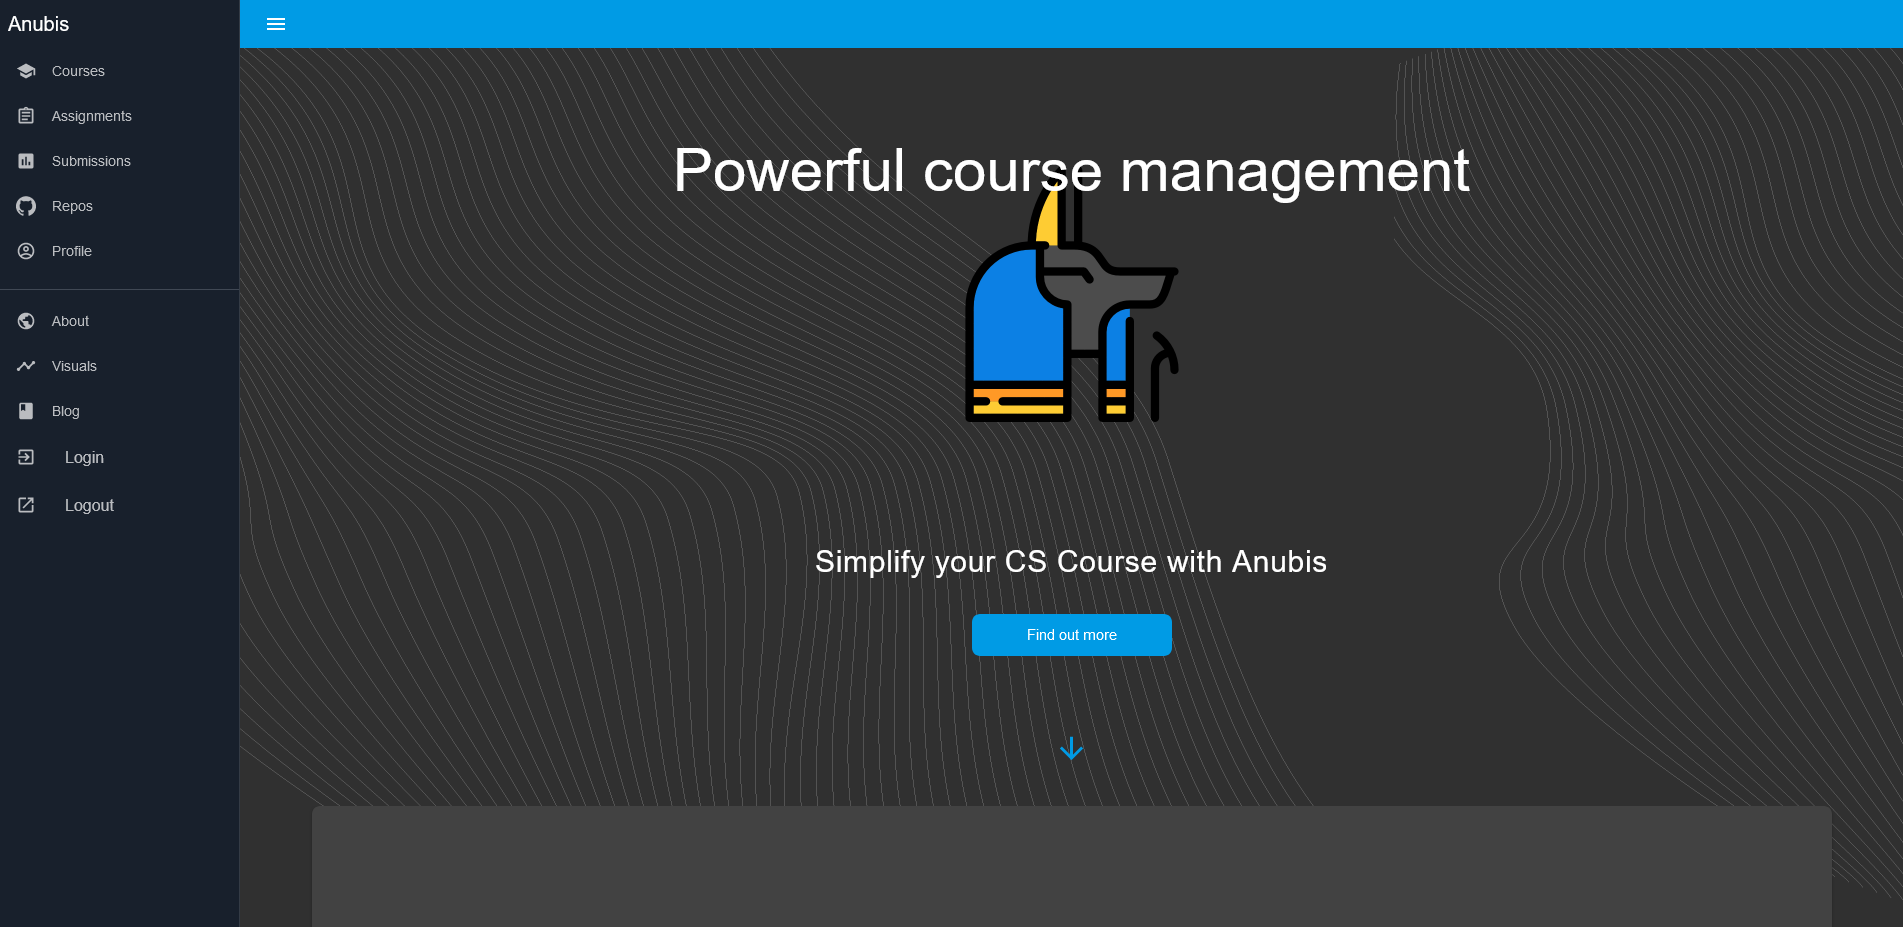
\includegraphics[width=0.75\textwidth]{figures/anubis-frontend}
    \caption{Anubis Web Frontend\label{fig:web-frontend}}
\end{figure}

The web static service is nothing more than a simple static http webserver.
There are no moving parts that are necessary for this service.
Only the compiled reactjs, html and css files are found in this service.
One thing of note that is not in this service are most images.
The only images that are in this web static image are the logo favicons
and some others.
The majority of images that are on the frontend (through the blog or assignment questions and whatnot)
are saved in the database and accessed through the api~\fref{sec:api}.

The frontend is designed to be a simple reflection of the backend data.
Once authenticated, users will be able to see the classes they are a part of, 
current and past assignments, and all their submissions. 
With few exceptions, the frontend is a near one to one translation of the API's data models.
Most pages will have a corresponding API endpoint. 
The data shown on that page will be in exactly the form of the API response.

\section{Anubis Theia Proxy}\label{sec:theia-proxy}

\section{RPC in Anubis}\label{sec:rpc-in-anubis}

\subsection{Default RPC}\label{sec:default-rpc}

\subsection{Regrade RPC}\label{sec:regrade-rpc}

\subsection{Theia RPC}\label{sec:theia-rpc}

